\documentclass[12pt]{article}

\usepackage{fullpage}
\usepackage[round]{natbib}
\usepackage{multirow}
\usepackage{booktabs}
\usepackage{graphicx}
\usepackage{float}
%\usepackage{../ltx/edcomms}
\usepackage{../ltx/setupComments}
\usepackage{hyperref}
\usepackage{geometry}
\usepackage{changepage}
\usepackage{adjustbox}
\usepackage{graphicx}
\usepackage[section]{placeins} % Prevents floats from floating across sections
\usepackage{tabularx}
\usepackage{amsfonts}
\usepackage{glossaries}
%\usepackage{amssymb}
\newcounter{acnum}
\newcommand{\actheacnum}{AC\theacnum}
\newcommand{\acref}[1]{AC\ref{#1}}

\newcounter{ucnum}
\newcommand{\uctheucnum}{UC\theucnum}
\newcommand{\uref}[1]{UC\ref{#1}}

\newcounter{mnum}
\newcommand{\mthemnum}{M\themnum}
\newcommand{\mref}[1]{M\ref{#1}}
\makeglossary
\begin{document}

\title{\vspace*{3cm} Module Guide for ECA Rules for Ampersand} 
\author{Yuriy Toporovskyy (toporoy)\\ Yash Sapra (sapray) \\ Jaeden Guo (guoy34)}
%%Yuriy Toporovskyy (toporoy) \\ Yash Sapra (sapray) \\ Jaeden Guo (guoy34)}
\date{February 24th,\ 2016} 


\maketitle
\newpage
\vspace*{1cm}
\begin{table}[ht!]\begin{center}
        \caption{Revision History}  
        \begin{tabular}{|c|c|c|}\hline
            \textbf{Author} & \textbf{Date} & \textbf{Comments} \\\hline 
            Yash Sapra & 24 / 02 / 2016 & Initial draft\\\hline
	 Jaeden Guo & 27/ 02 / 2016 & Update and merge \\\hline
        \end{tabular}
    \end{center}\end{table}
\newpage

\tableofcontents

\newpage

\section{Introduction}
%TODO: edit for grammar, spelling, context, flow, watch for contractions
\subsection{Description}
The document outlines the design decision for the EFA project. 
EFA is responsible for generating SQL Statements from ECA rules that will 
be used to fixed any data inconsistencies in the Ampersand Database.

This document follows the principle set by Parnas and Clements\citep{fakeIt}. 
EFA is currently in development where changes occur frequently, a 
commonly accepted practice for this situation is to decompose modules based on 
the principle of abstraction, where unnecessary information in hidden for the 
benefit of designers and maintainers\citep{modStruct,Parnas1972}.
 
Our design follows the principles laid out by \citep{modStruct}, as follows:
\begin{itemize}
\item Unnecessary design details are omitted for simplicity
\item Each data structure is only in one module
\item Any other program that requires information stored in a module's data
  structures must obtain it by calling access programs belonging to that module.
Additionally: 
\item Each module is broken down based on hierarchy
\item Reference material are provided for external libraries but details of its 
use will not be provided within the module break-down
\end{itemize}

\subsection{Scope}
This project aims to improve upon the current Ampersand system by providing a 
permanent replacement for the exec-engine. EFA automatically restores system 
invariants according to ECA rules with no manual maintenance required.

\subsubsection{Intended Audience}
This document is designed for:
\paragraph{New project members:}
This document designed to be a guide to introduce new Ampersand users to EFA 
(ECA rules for Ampersand). It provides a basic structure that allows 
individuals to quickly access what they are looking for.
   
\paragraph{Maintainers \& Designers:} The structure of this module guide will 
help maintainers rationalize where changes should be made in order to 
accomplish their intended purpose. Furthermore, the design document will act as 
a guide to EFA for future designers of Ampersand.

\section{Anticipated and Unlikely Changes}
\subsection{Anticipated Changes}
It is likely that EFA will require changes to the front-end interface and an 
addition that will connect the front-end interface to back-end functions, which 
will give the user more control. In addition, ECA rules are not static and may 
change over time, if changes do take place those changes will need to be 
incorporated into EFA's future versions. 

Thus far anticipated changes include:

\begin{description}
    \item[AC1:] New front-end interface.
    \item[AC2:] Addition or elimination of ECA rules.
    \item[AC3:] The algorithm used for EFA.
    \item[AC4:] The format of output.
    \item[AC5:] The format of input parameters.
    \item[AC6:] The format of initial input data and associated markers for 
    data association.
    \item[AC7:] Integration of front-end interface to back-end modules.
    \item[AC8:] Implementation of SQL data structure
    \item[AC9:] Testing for individual modules and internal systems
    \item[AC10:] Software requirements for running Ampersand and by extension 
    EFA
    
\end{description}

\subsection{Unlikely Changes} 

These unlikely changes include the things that will remain unchanged in the 
system, and also changes that would not affect EFA. 

\begin{description}
    \item[UC1:] There will always be a source of input data external to the 
    software. 
    \item[UC2:] Results will always be provably correct. 
    \item[UC3:] The goal of EFA is to automatically correct system invariants
    \item[UC4:] Output data must exist
    \item[UC5:] The implementation language must be the same as that which is 
    used for building the Ampersand system
    \item[UC6:] The format of initial input data and associated markers for 
    data association. 
    \item[UC7:] Type of output data will always be SQL.
\end{description}

\section{Module Hierarchy}
This section provides an overview of the module design. Modules are decomposed 
based on their hierarchy from top to bottom. The modules are broken down into 
three sections, the first section consists of the main module used for EFA, 
the second section contains support modules and finally the last section
contains external libraries.

\begin{description}
    \item[M1:] eca2SQL
    \item[M2:] TypedSQL
    \item[M3:] Equality
    \item[M4:] Singletons
    \item[M5:] Utils
    \item[M6:] Trace
    \item[M7:] Combinators
    \item[M8:] Pretty
\end{description}

\begin{figure}
    \centering
    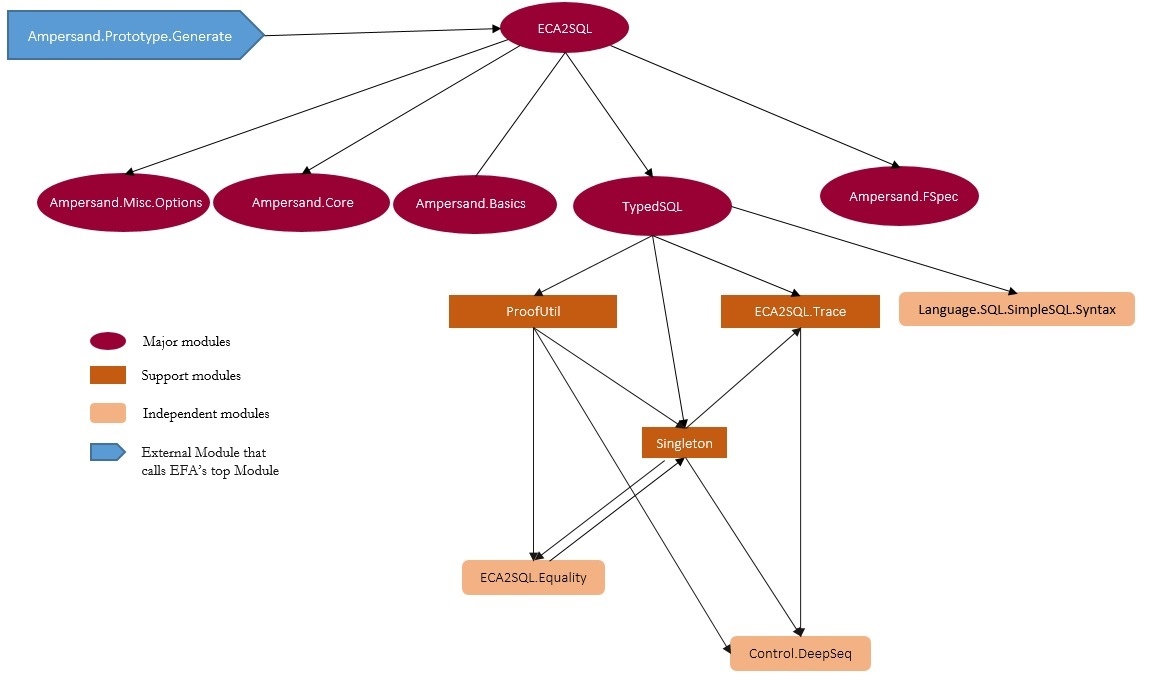
\includegraphics[width=0.95\textwidth]{../DesignDoc/depent_tree}
    \caption{Dependency graph of EFA modules}~\label{fig:figure1}
\end{figure}

\section{Connection Between Requirements and Design} \label{SecConnection}

\section{Module Decomposition} \label{SecMD}
Modules are located in their respective subsections (i.e. main module, support 
modules and external library modules). Each module is decomposed based on their 
use while hiding implementation details. 
\\ \newline
\textit{Please see glossary for math references and clarification of uncommon 
terms}

\subsection{Main Module}

%% ------------------------------M1: ECA2SQL -------------------------------%%
{\setlength{\tabcolsep}{6pt} 
    \begin{tabularx}{\textwidth}{>{\bfseries}m{3cm}X}
        M1 & eca2SQL \\ 
        \midrule 
        Main function & eca2SQL
        \\  Input & Options, FSpec, ECARule
        \\  Output & Doc
        \\	Secrets & The algorithm and data structures used to implement ECA 
        Rules.
        \\	Services & Produces the final product by using supporting modules 
        as tools in translating ECA rules to SQL statements which can be 
        applied to a database.
        \\     
         \vspace{12pt}
     \end{tabularx}
\\
\underline{Internal Description}\\ \\
eca2SQL :: Options $\rightarrow$ FSpec $\rightarrow$ ECArule $\rightarrow$ Doc

%% ------------------------------M2: TypedSQL -------------------------------%%
\subsection{Support Modules}

{\setlength{\tabcolsep}{6pt} 
    \begin{tabularx}{\textwidth}{>{\bfseries}m{4cm}X}
        M2 & eca2SQL \\ 
        \midrule       
        \\  Requires Modules & ProofUtils, Trace, Singleton
        \\	Secrets & Implements a type language for SQL through pattern 
        matches where the representation of SQL references types which can 
        appear in SQL statements.
        \\	Services & Contains Base which implements a typed SQL query 
        language and a type SQL statement.
        \\         
        \vspace{12pt}
    \end{tabularx} 


\setlength{\parindent}{0pt}
\underline{Internal Description}\\

Read as: \textit{function: input $\rightarrow$ input2 $\rightarrow$ 
output}\newline

Where a function may require multiple inputs of different types to produce the 
necessary output type.\\

\textit{function (type and value level): (x:A) $\rightarrow$ output}
This indicates the function of a certain type and its value level, this is seen 
on SQL types. (x:A) is used to indicate a variable x of type A (e.g. x=9, (x:A) 
is a type of integer). (function::) is used to define a function and its input 
types 



\newglossaryentry{N}{name=N, description= $\mathbb{N}$ represents 
    the 
    set of natural numbers}

 (:::) : Symbol $\rightarrow$ SQLType $\rightarrow$ SQLRecLabel \\
 
 SQLSizeVariant : Kind \\
 SQLSmall, SQLMedium, SQLNormal, SQLBig :SQLSizeVariant \\ \\
 
 SQLSign : Kind \\
 SQLSigned, SQLUnsigned : SQLSign  \\
 
 SQLNumeric : Kind \\
 SQLFloat, SQLDouble : SQLSign $\rightarrow$ SQLNumeric \\
 
 SQLInt : SQLSizeVariant $\rightarrow$ SQLSign $\rightarrow$ SQLNumeric \\
 SQLRecLabel : Kind \\

 SQLType : Kind \\
 SQLBool, SQLDate, SQLDateTime, SQLSerial : SQLType \\
 
 SQLNumericTy : SQLNumeric $\rightarrow$ SQLType  \\
 SQLBlob : SQLSign $\rightarrow$ SQLType \\
 
 SQLVarChar : \Gls{N} $\rightarrow$ SQLType 
 SQLRel : SQLType $\rightarrow$ SQLType \\
 
 SQLRow : [SQLRecLabel] $\rightarrow$ SQLType 
 SQLVec : [SQLType]$\rightarrow$ SQLType \\
 
 SQLRef, SQLUnit: SQLType \\
 SQLRefType: Kind\\
 
 SQLMethod: [SQLType] $\rightarrow$ SQLType $\rightarrow$ SQLRefType \\
 SQLVal: SQLType $\rightarrow$ Type \\
 
 SQLScalarVal: IsScalarType a $\equiv$ True $\rightarrow$ Sm.ValueExpr 
 $\rightarrow$ SQLVal a \\
 SQLQueryVal: IsScalarType a $\equiv$ False $\rightarrow$ Sm.QueryExpr 
 $\rightarrow$ SQLVal a \\
 
 SQLValSem: SQLRefType $\rightarrow$ Type\\

 
 Ty: SQLType $\rightarrow$ SQLRefType \\

 IsScalarType: SQLType $\rightarrow$ Bool \\
 isScalarType: (x:SQLType) $\rightarrow$ IsScalarType x \\
 IsScalarTypes: [SQLType] $\rightarrow$ Bool \\
 isScalarTypes: (X:[SQLType]) $\rightarrow$ IsScalarTypes x \\
 
 typeOf: SQLVal a $\rightarrow$ a \\
 argOfRel: SQLRel a $\rightarrow$ a\\
 
 Unit: SQLValSem SQLUnit\\
 Val:: SQLVal x $\rightarrow$ SQLValSem ('Ty x)
 
 

%% ------------------------------M3: Equality -------------------------------%%
{\setlength{\tabcolsep}{6pt} 
    \begin{tabularx}{\textwidth}{>{\bfseries}m{4cm}X}
        M3 & Equality \\ 
        \midrule
        
        Contains functions  &  not, cong, elimNeg and more
        \\	Secrets & Various utilities functions
        \\	Services &  The module contains utility functions that are being used in the Singletons and Utils module to provide type level security for the TypedSQL with an aim to make it total.
        \\       
        \vspace{12pt}
    \end{tabularx}
    \vspace{3em}
%% ------------------------------M4: Singleton -------------------------------%%
{\setlength{\tabcolsep}{6pt} 
    \begin{tabularx}{\textwidth}{>{\bfseries}m{4cm}X}
        M4 & Singleton \\ 
        \midrule
        
        Main function  &  No functions exported
        \\	Secrets & Extension to the Haskell Singleton Library Singleton Types and promoted functions
        \\	Services &  
        \\       
        \vspace{12pt}
    \end{tabularx}\vspace{3em}
%% ------------------------------M5: Utils -------------------------------%%
{\setlength{\tabcolsep}{6pt} 
    \begin{tabularx}{\textwidth}{>{\bfseries}m{4cm}X}
        M5 & Utils \\ 
        \midrule
        
        Main function  & 
        \\	Secrets & Varies Utilities Functions
        \\	Services &  The module also contains some utility functions used by the ECA2SQL module
        \\       
        \vspace{12pt}
    \end{tabularx}\vspace{3em}
%% ------------------------------M6: Trace -------------------------------%%
{\setlength{\tabcolsep}{6pt} 
    \begin{tabularx}{\textwidth}{>{\bfseries}m{4cm}X}
        M6 & Trace \\ 
        \midrule
        
        Main function  &  getTraceInfo 
        \\	Secrets & Creates a function for tracing the output
        \\	Services &  The modules contains support for tracing back the ECA rule. Tracing is used for development and debugging purpose
        \\       
        \vspace{12pt}
    \end{tabularx}\vspace{3em}
%% ------------------------------M7: Combinators------------------------------%%
{\setlength{\tabcolsep}{6pt} 
    \begin{tabularx}{\textwidth}{>{\bfseries}m{5cm}X}
        M7 & Combinators \\ 
        \midrule
        
        Main function  & No functions exported
        \\	Secrets &  Combinator Logic for TypedSQL
        \\	Services &  This module contains Combinatory Logic for our TypedSQL module. The module defines SQL primitives such as AND, OR, NOT and the primitive SQL functions such as the EXISTS, GROUP BY, SORT BY.
        \\       
        \vspace{12pt}
    \end{tabularx}\vspace{3em}
%% ----------------------------- M8: Pretty    ------------------------------%%
    {\setlength{\tabcolsep}{6pt} 
        \begin{tabularx}{\textwidth}{>{\bfseries}m{5cm}X}
            M8 & Pretty \\ 
            \midrule
            
            Main function  & eca2PrettySQL
            \\	Secrets & Pretty prints the generated SQL
            \\	Services &  The function takes in the FSpec as an input with an ECA rule and runs the eca2SQL function to generate SQLSt(SQL Statements). The generated SQL statement are pretty printed using a Pretty Printer Library.
            \\       
            \vspace{12pt}
        \end{tabularx}\vspace{3em}
\underline{Internal Description}\\ \\
eca2PrettySQL :: Options $\rightarrow$ FSpec $\rightarrow$ ECArule $\rightarrow$ Doc
        
\subsection{External Libraries}
\begin{tabular}{ | m{4cm} | m{11cm} |}
    \hline
    \bfseries{Library} & \bfseries{Reference}  \\
    \hline
    item 21  & item 22   \\
    item 21  & item 22   \\
    item 21  & item 22   \\
    item 21  & item 22   \\
    \hline
    \end{tabular}

\section{Traceability Matrix} \label{SecTM}

\section{Use Hierarchy Between Modules} \label{SecUse}





%\section*{References}
\clearpage
\printglossaries
\bibliographystyle {plainnat}
\bibliography {docDesign}

\end{document}